\chapter{Grundlagen}
In den einleitenden Abschnitten wurden bereits einige Begriffe verwendet, die noch nicht zur Gänze erklärt sind bzw. die für das Verständnis der Entwicklungsgeschichte und auch für den technischen Gesichtspunkt wichtig sind.

Dazu gehören Ontologien, für was sie stehen und wozu sie nützlich sind. Die Beschreibung des OWL2 RL Fragments. Das Verständnis für einen Schlussfolgerer, sowie einige Hintergründen für die Umsetzungen von Ontologien in Datenbanken.

\section{Kriterien der Wissensrepräsentation}

Die Wissensrepräsentation ist zentraler Bestandteil eine KI-Systems. Eine Wissensrepräsentation wird zu jedem Bereich von intelligenten rechnergestützten Systemen benötigt.

Eine Wissensrepräsentation kann für verschiedene Anwendungsgebiete ausgelegt sein, daher gibt es einige allgemeine Kriterien, um solche Sprachen einzuordnen.

Die wichtigsten Begriffe zur Einordnung dabei sind:
\begin{itemize}
  \item Korrektheit
Ein Verfahren ist korrekt, wenn es nicht möglich ist falsche Schlüsse aus einer Wissenrepräsentation zu ziehen. Falsche Schlüsse beziehen sich dabei auf die Semantik des Verfahrens.
 \item Vollständigkeit
Ein Verfahren ist vollständig wenn alle korrekten Schlüsse folgerbar sind.
 \item Entscheidbarkeit
Ein Verfahren ist entscheidbar, wenn immer der Algorithmus für das Schlussfolgern immer existiert.
 \item Adäquatheit
Eine Wissensrepräsentation ist adäquat, wenn die Formulierung von Problemen auf eine einfache und verständliche Art möglich ist.
 \item Komplexität
Die Komplexität beschreibt den theoretischen minimalen Aufwand für den Schlussfolgerungs-Alogrithmus
\end{itemize}


\subsection{OWL2 RL Eigenschaften}
Das OWL2 RL Sprachfragment wurde speziell für Anwendungsgebiete entwickelt, die die größtmögliche Ausdrucksmächtigkeit benötigen, ohne dabei die Eigenschaft verlieren effizient ableitbar zu sein. Effizient ist dabei sehr theoretisch zu verstehen. Solange die Ableitungsfunktion in polynomieller Die Sprachuntermenge von OWL2 wurde dabei so gewählt, das sie günstig mit einem regelbasierten Ansatz abzuleiten ist. Dazu wurde auch direkt Inferenzregeln angegeben die diesem Fragment eine Semantik gibt. Der Entwurf dieses Sprachfragement wurde dabei von DLP [ref] und pD* [ref] inspiriert.

Damit fällt OWL2 RL auch in die Kategorie der monotonen Sprachen, das bedeutet wenn neue expliziten Fakten zur Wissensbasis hinzugefügt werden, diese neue implizite Fakten zur Wissenbasis hinzufügen. Aber unter keine Umständen können die expliziten Fakten das Entfernen von bereits abgeleiten Fakten verursachen. Damit kann das Hinzufügen von neuen Fakten die abgeleitete Wissenbasis nur monoton erweitern. [ref englischer Text aus dem Wiki]

Um einige geschwünschte Eigenschaften für die Sprache zu erhalten ist es dabei nötig nicht nur die verwendeten Konstrukte einzuschränken, sondern auch die Syntax. Daazu wird in OWL2 RL eine Grammatik vorgegeben, an welcher Stelle welche Konstrukte verwendet werden dürfen.

Sofern sich eine Ontologie an die syntaktischen Rahmenbedigungen des Sprachfragments hält und ein Schlussfoglerer entsprechend der angebenen Regelsemantik implementiert ist, können sich daraus einige positive Kriterien ableiten lassen. So ist dann garantiert, das alle und nur gültige Ergebnisse vom Schlussfolgerer geliefert werden. Das Verfahren für die Wissensrepräsentation ist damit korrekt und vollständig. (siehe Beweis)
Mit dieser regelbasierten Implementierung ist es sogar möglich in nicht-syntaktisch konformen Ontologien zu schlussfolgern. Es ist dann zwar nicht mehr möglich alle Ergebnisse zu ermitteln, aber es werden zumindest weiterhin nur gültige Ergebnisse abgeleitet. [ref wc3]

Eine montone Logik ist besonders wichtig für den Einsatz im Web. Hier werden viele kleine verteilte Wissensbasen erzeugt. In einer Sammlung solcher Wissensbasen kann dann geschlussfolgert werden. Wird diese Sammlung erweitert, verkleinert oder verändert ist es natürlich umständlich wenn wieder über alle anderen Beziehung geschloßen werden müsste. Durch eine montone Logik ist eine modulare Umsetzung besonders gut zu realisieren.

Eine vollständige Beschreibung für die syntaktisch Einschränkung dieser Sprache findet man im Anhang und in der Referenz [ref].

\subsection{Sprachkomplexitäten}
Im folgenden werden verschieden Sprachen an Hand ihrer Komplexität kurz gegenüber gestellt, um einen Vergleichsbasis zu haben.

\subsubsection{Attributive Language}
Die attributive language ist die grundlegende Beschreibungssprache. Sie wird mit $\mathcal{AL}$ abgekürzt und enthält folgende Operatoren für ihre Ausdrucksmöglichkeiten.

$\mathcal{AL}$: C,D $\Longrightarrow$ A | $\top$ | $\bot$ | $\lnot$A | C $\land$ D | $\forall$r.C | $\exists$r

Diese attributive language kann durch weitere Operatoren in ihrere Ausdrucksmächtigkeit vergrößert werden. Für die Menge an Möglichkeiten hat sich dabei ein Namensschema herauskristallisiert. Dies ist zwar kein offizielles und eindeutiges Schema wird aber von vielen Programmen wie z.B. Protégé verwendet.

Bei diesem Namenschema werden an die Buchstaben AL noch weitere Kürzel angehängt die für die zusätzlichen Operatoren stehen.
\begin{itemize}
  \item $\mathcal{C}$ für volle Negation (Complement)
  \item (D) für konkrete Domänen\newline
Damit ist der Einsatz von Literalen möglich, z.B. in datatype properties, data values oder data types.
  \item $\mathcal{U}$ Konzeptvereinigung (Union)
  \item $\mathcal{E}$ Existenzquantoren für komplexe Ausdrücke (Exists)\newline
Existenzquantoren sind an für alle Arten von Ausdrücken erlaubt.
  \item $\mathcal{N}$ Kardinalitätseinschränkungen.
  \item $\mathcal{I}$ Inverse Eigenschaften (Inverse)
  \item $\mathcal{O}$ Aufzählungen von object values (Nominals)
  \item $\mathcal{H}$ Hierarchie von Eigenschaften (Role hierarchy)
  \item $\mathcal{F}$ Funktionale Eigenschaften
\end{itemize}
\cite{wiki:DL}

\subsubsection{Komplexität in Form der attributive language}
\begin{itemize}
  \item U2R2 basiert auf der DLP Sprache und ist damit ein Reasoner auf der $\mathcal{ALCHIF}$-Sprache ($\mathcal{SHIF}$)
  \item Die Sprache OWL1 bzw. OWL-DL liegt in $\mathcal{ALCHOIN}$ ($\mathcal{SHOIN}$)
  \item OWL2 basiert auf $\mathcal{ALCROIQ}$ ($\mathcal{SROIQ}$) \cite{Krötzsch2008}
\end{itemize}


TABELLE der Komplexitäten TABELLE
\begin{table}
	\rowcolors{3}{lightgray}{white}
	
	\begin{tabular}{|m{1.4cm}|p{2cm}|p{2cm}|p{2cm}|p{2cm}|p{2cm}|}
	\hline
	Sprache & Schlussfolger\-ungs\-problem & Komplexität der Taxonmie & Daten\-komplexität & Abfrage Komplexität & Kombinierte Komplexität \\
	\hline
	\hline
	\multirow{2}{*}{OWL-DL} & Ableitung & NEXPTIME-vollständig & Offen & Nicht anwendbar & NEXPTIME-vollständig \\ \cline{2-6}
		& Abfragen & Offen & Offen & Offen & Offen \\
	\hline
	\multirow{2}{*}{DLP} & Ableitung & In EXPTIME & PTIME-vollständig & Nicht anwendbar & In EXPTIME \\ \cline{2-6}
		& Abfragen & In EXPTIME & PTIME-vollständig & In EXPTIME & In EXPTIME \\
	\hline
	\multirow{2}{*}{OWL2 Direct Semantics} & Ableitung & 2NEXPTIME-vollständig & entscheidbar, aber Komplexität offen & Nicht anwendbar & 2NEXPTIME \\ \cline{2-6}
		& Abfragen & Entscheidbarkeit offen & Entscheidbarkeit offen & Entscheidbarkeit offen & Entscheidbarkeit offen \\
	\hline
	\multirow{2}{*}{OWL2 EL} & Ableitung & PTIME-vollständig & PTIME-vollständig & Nicht anwendbar & PTIME-vollständig \\ \cline{2-6}
		& Abfragen & PTIME-vollständig & PTIME-vollständig & NP-vollständig & PSPACE-vollständig \\
	\hline
	\multirow{2}{*}{OWL2 QL} & Ableitung & NLogSpace-vollständig & In AC$^0$ & Nicht anwendbar & NLogSpace-vollständig \\ \cline{2-6}
		& Abfragen & NLogSpace-vollständig & In AC$^0$ & NP-vollständig & NP-vollständig \\
	\hline
	\multirow{2}{*}{OWL2 RL} & Ableitung & PTIME-vollständig & PTIME-vollständig & Nicht anwendbar & PTIME-vollständig \\ \cline{2-6}
		& Abfragen & PTIME-vollständig & PTIME-vollständig & NP-vollständig & NP-vollständig \\
	\hline
	\end{tabular}
	
	\cite{WebontTractable}
	\cite{OWL2Complexities}
	\cite{ComplexityNavigator}
\end{table}

Natürlich ist das Sprachfragemnt OWL2 RL entscheidbar und zwar in polynomieller Zeit entscheidbar. In der Profilbeschreibung wird dabei feiner unterschieden.

\subsection{Zusammenhang mit einem Schlussfolgerer}
%besser in Konzeption oder Realisierung
Die Wissensrepräsentation hängt nicht direkt mit dem Schlussfolger zusammen, wenn man allerdings über die gewünschte Wissensrepräsentation bescheid weiß, ist es möglich den Schlussfolger daraufhin zu trimmen. Im Falle dieser Arbeit wird mit einer Wissensrepräsentation gearbeitet -- OWL2 RL -- und der Schlussfolgerer ist daraufhin optimiert, die in der Sprache repräsentierten Kriterien, wie Entscheidbarkeit und Komplexität zu erreichen.
Das bedeutet zum einen einfach, das wenn die Sprache entscheidbar ist, also es einen immer einen terminierenden Alogrithmus gibt. Das ist durch zwei Dinge zu erreichen, ein gutes Design, welches diesen Algorithmus überhaupt ermöglicht und eine fehlerfreie Programmierung. Diese beiden Dinge sind natürlich nie so in der Praxis zu ereichen, aber es wurde versucht den Code und die Architektur so einfach und verständlich wie möglich zu halten, um Fehler schnell zu finden.
Die Komplexität einer Sprache gibt nur einen theoretischen Wert an, der für eine Lösungsfindung nötig ist. Die Umsetzung in einem Programm muss diesen dann erst noch erreichen. Das wird im hier behandelten Schlussfolgerer versucht zu erreichen, indem man sich nur auf eine Wissensrepräsentation konzentriert. Damit können die Regeln zur Wissensgewinnung nah an der Definition der Sprache umgesetzt werden und somit auch nah an der theoretischen Komplexität bleiben.
Die anderen Kriterien spielen für den Schlussfolgerer nur eine untergeordnete Rolle.

\section{Ontologien}
= Unterschied zu relationaler Datenbank =

Beim Abspeichern einer Ontologie in einer relatioalenDatenbank sind zwei konzpetionelle Dinge zu beachten. In einer Ontologie gilt die unique name assumption, das bedeutet das in der Ontologie verwendete Namen zum identifizieren von  eindeutig sind und sicher immer auf die selbe Entität beziehen. In einer Relation ist das nicht zwingend vorausgesetzt. Nur wenn Spalten als Schlüssel oder unique deklariert werden wird sichergestellt das Namen eindeutig sind.
Der zweite Unterschied besteht darin, wie man über die Daten schließt. In einer Datenbank geht man davon aus, das man die komplette Welt modelliert hat und alle Fakten vorhanden sind. Kann etwas nicht gefunden werden ist nicht Tel des Modells und damit falsch. In einer Ontologie werden Fakten, die nicht vorhanden sind als unbekannt eingestuft. Sie sind damit weder wahr noch falsch.
\begin{figure}
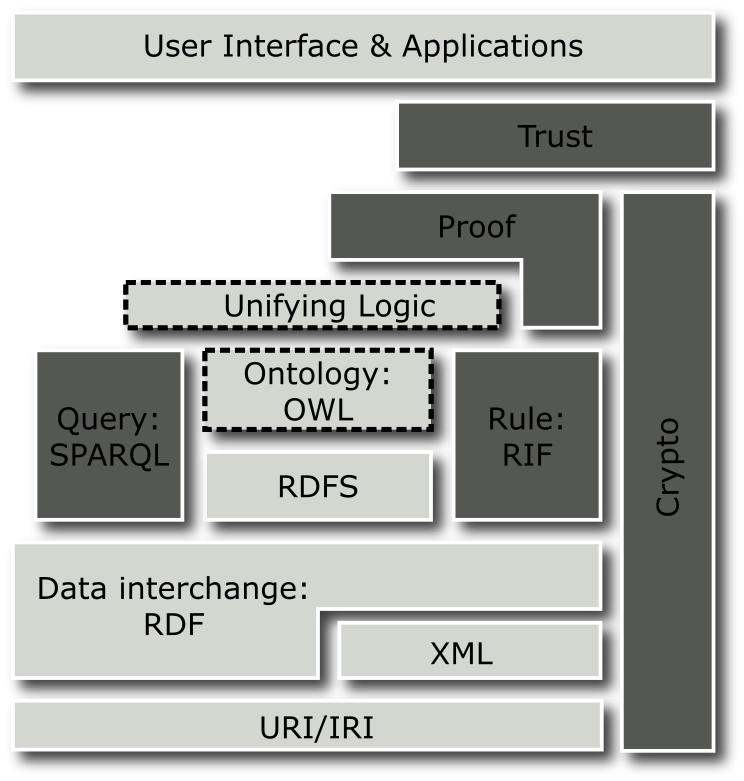
\includegraphics{images/w3-layercake.pdf}
\end{figure}

\section{OWL2}
 http://www.cs.man.ac.uk/~sattler/publications/sroiq-TR.pdf
OWL2 DL liegt in SROIQ
gefunden in  http://www.w3.org/TR/2009/REC-owl2-overview-20091027/
2.3 Semantics
\begin{figure}
\includegraphics{images/owl-layer-map.pdf}
\end{figure}

\begin{figure}
\includegraphics{images/sprachhierarchie.pdf}
\end{figure}

\begin{figure}
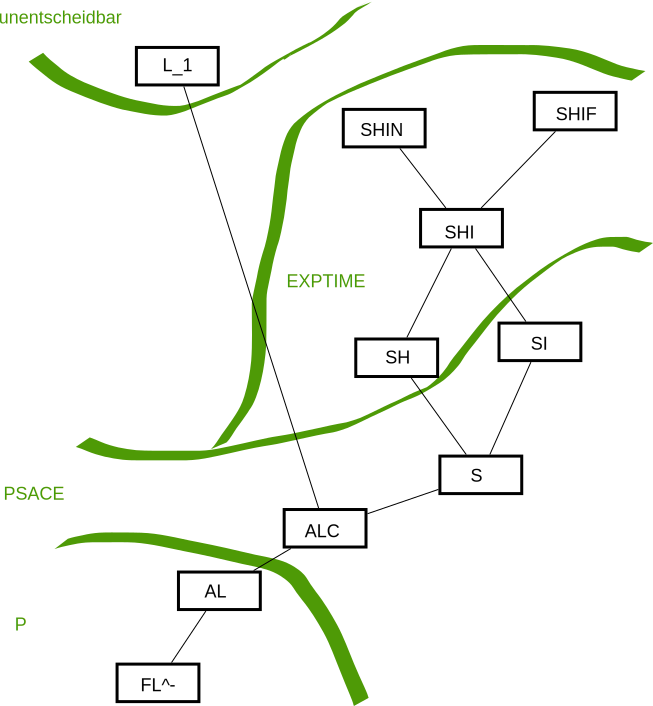
\includegraphics{images/sprachkomplexitaeten-wimo-blatt4.pdf}
\end{figure}

\section{Schlussfolger}

\section{U2R2}

\section{Aktueller Stand auf dem Onto-Gebiet}
Nicht nur die aktuelle Veröffentlichung der OWL2 Spezifikation zeugt davon das im Moment die Entwicklung im Ontologie-Bereich der künstlichen Intelligenz in vollem Gange ist. Auch auf der Seite des W3C für Semantic Web findet man eine große Anzahl an Projekten die auf dieser Basis arbeiten.
Darunter sind z.B.:
\begin{itemize}
  \item AUFZÄHLUNG USE CASES
\end{itemize}
Diese verschiedenen Bereiche zeigen auf das Ontologien einerseits unterschiedliche Bereiche verbinden aber auch ihrer Wichtigkeit.

OWL2 wurde erst im Verlaufe dieser Diplomarbeit als Recommendation veröffentlicht, aber die Weiterentwicklung von OWL ist auch schon in Planung [ref OWL3 Suggestions] und es werden verschieden Konferenzen zu diesem Thema abgehalten.
\begin{itemize}
  \item AUFZÄHLUNG VON KONFERENZEN
\end{itemize}

\begin{verbatim}
    * Was ist OWL im Hinblick auf Ontologien?
         o Wo ist das OWL2 RL Fragment einzuordnen?
          o Wie ist OWL2 aufgebaut?
          o Was sind andere Profile
          o Was sind ihre Unterschiede
          o Was sind ihre Eigenschaften.
    * Was ist interessant bzgl des Fragements OWL2 RL?
    * Was ist das Einsatzgebiet von OWL2 RL?
    
    * Wie ist der OWL2 Zeitplan?
    
    * Warum braucht man einen Reasoner?
    * Was zeichnet einen Reasoner aus? Welche Funktionen muss er bereitstellen?
    
    * Was ist die Herkunft und der Hintergrund meiner DA?
    * Wie ordnet sich U2R2 ein? Was ist der Reasoner Ansatz/ die Reasoner Strategie?
    * Wie war dieser Reasoner aufgebaut und konzipiert?
    * Was waren die Fähigkeiten von U2R2?
\end{verbatim}
